\startchapter{Evaluation of Word Vectors using BrainBench V2.0}
\label{chapter:newsol}

The previous chapter discussed in detail about major contributions made in the field of study of representations of language. It also explained in depth about various Distributional Semantic models (DSM) or word vectors trained on text corpora and how Computational linguists use these models to study semantic representation in the human brain. The previous chapter also discussed about \textit{BrainBench}- a system designed to test, evaluate and benchmark word vector models using brain data \cite{BrainBench2016}. \textit{BrainBench} reported comparable performance to other systems which evaluate and benchmark DSM's.



However, BrainBench tests include just 60 concrete nouns.  Nouns only form a small subset of various parts of speech that constitutes the language. Another limitation is that the tests do not include any abstract nouns. Moreover, the tests are derived from only two dataset sources (a fMRI and a MEG) and based on one language (English). Considering that DSM's are available in multiple languages and not including brain data from other language sources as a part of BrainBench tests is a serious limitation. 

To address these limitations, we release the second iteration of BrainBench (V2.0) which introduces two new datasets (an fMRI and an EEG dataset collected from Italian participants) to BrainBench tests. This improves the coverage of the tests from 60 words to 190 words. The Italian fMRI introduces abstract nouns to the test suite. We also evaluate the performance of word vectors trained on non-English corpora using our Italian Brain datasets. Then we compare the performance of word vectors on abstract nouns and concrete nouns separately.

Traditionally, EEG data was not recommended for studying semantics in Brain due to its poor Signal to Noise ratio (SNR). However, the work of Murphy et al \cite{MurphyEEG} provided strong argument that EEG dataset along with semantic models could be used for studying semantics in Brain. The results of our experiments with EEG dataset further reinforces this argument. EEG has higher temporal resolution and makes it ideal for studying word comprehension and semantic representation in brain. EEG is more portable and much cheaper as compared to fMRI, making it ideal for experiments.




Anderson et al. studied the performance of  the performance of image-based semantic models against against anatomical regions in human brain \cite{andersonBrainEyes}. However, the semantic models and the methodology used in our study are different to their study. We incorporate into BrainBench the ability to study word vector performance across various anatomical region in human brain. This is discussed in detail under the section \textit{Evaluation against anatomical brain region} of this chapter.

The contributions to BrainBench addressed by this chapter are summarized below.

\begin{itemize}

\item {Introduction of abstract nouns into the BrainBench tests and evaluation of performance of various word vectors on abstract nouns.}
\item{Addition of Italian Brain data into BrainBench and study of performance of non-English word vectors.}
\item {Addition of an EEG dataset to BrainBench.}
\item {The study of performance of word vectors across various Brain regions using Brain Atlas mapping collected using fMRI.}
\end{itemize}

\section{Brain Datasets}
%Give a three line Introduction
In this section, we discuss in detail about the four brain datasets that are used as a part of BrainBench test suite. We primarily focus on the data collection techniques, concept selection and brain signal preprocessing for each of the below datasets.

\subsection{Data Science fMRI}

\subsection{Data Science MEG}

\subsection{Italian fMRI}
This dataset was released as part of the experiments conducted by Anderson et al. to study the varying degree of concreteness in taxonomic categories in human brain using fMRI. Brain signal was collected from nine native Italian speakers viewing 70 concepts on a screen and imagining it. The 70 concepts selected were from two domains \textit{music} and \textit{law}. Moreover, these 70 concepts were organized into 7 Taxonomic categories (Attribute, Communication, Event, Social Role, Tool, Location and Urabstracts) using MultiWordNet (the Italian version of WordNet \cite{wordnet})~\cite{ItalianWordNet}. This resulted in 70 stimuli with 10 concepts from each taxonomic categories. Music and law domains had five words each within each taxonomic category. The selection of the concepts were done in such a way that there was a varying degree of concreteness with tool being the most concrete  and Urabstracts being the most abstract taxonomic category. 

The concreteness rating was assigned using word norming \cite{Barca2002WordNT} where 24 native Italian speakers were asked to rate the 70 concepts on a concreteness scale of 1 (highly abstract) to 7 (Highly concrete). The collected data was binarized as concrete=1 and abstract =0. The concepts and it's concreteness are summarized by the Figure:~\ref{BrainBenchMethod}.
\subsection{EEG}

\section{Distributional Semantic Models (DS)}
We evaluate five popular Distributional Semantic models as a part of our analysis. These models trained with different methodologies and corpus are described in detail below.

\noindent \textbf{Word2Vec and skip-gram:} The Word2vec model is probably the most widely
used model in NLP tasks. It was proposed by Mikolov et al. in
2013 and uses a shallow neural network to learn the embedding
space \cite{Word2Vec}. It consists of two distinct algorithms, a continuous bag
of words (CBOW) and Skip-gram model. A CBOW model was
trained to predict a target word from a set of contextual words
surrounding it. In vector space, this can be visualized as
predicting the distance between two different word vectors
which are in context to one another. For Skip-gram, the
direction of prediction is reversed, i.e. from a source word it
tries to predict all the words which are in context to the source
word. The skip-gram model trained on Google
news dataset is a 300-dimensional vector. We use the pre-trained skip-gram word vector available as a text file for our analysis.


\noindent \textbf{Glove:} is a regression based semantic model published by Pennington et al. in 2014 \cite{Glove}. It utilizes a word co-occurrence matrix rather than the actual text as input to train the model.  The intuition behind this model was that the semantic information in the word could be represented as the ratio of the co-occurrence probabilities of two words rather
than the co-occurrence probabilities itself (The method used by Word2vec). This  300 dimensional vector model was trained on a combined corpus of Wikipedia and Gigaword 5.

\noindent \textbf{Global Context:} This model takes into account both local
and global context of a document to learn the semantics of the word (Huang et al.;2012)~\cite{GlobalContext}. The model learns multiple embeddings per word to take into account of homonymy  and polysemy. Homonymy refers to the relation between words with identical forms but different meanings and polysemy is the the coexistence of many possible meanings for a
word or phrase. These embeddings are weighted averaged to produce a single vector of 50 dimensions per word and is trained on Wikipedia.


\noindent \textbf{Cross-lingual}: This model, proposed by Faruqui
and Dyer, 2014, takes into account semantic
properties across various languages \cite{Crosslingual}. It was trained using both German and English words using WMT-2011 corpus and uses a shared semantic space to learn the word embeddings. The resulting word vector
has 512 dimensions and is available as pre-trained text file.

\noindent \textbf{RNN:} A Recurrent Neural Network (RNN) trained  to predict the next word in the sequence (Mikolov et
al., 2011) \cite{RNN}. Unlike Skip-gram and other models which derives word
embeddings from an n-gram of words (Three or four words
which occur together), RNN model can theoretically
encode words which are in infinite distance to one another. This model trained on broadcast news transcriptions has a dimension of 640 for its word embeddings.

\noindent \textbf{Non-Distributional:} This semantic model was created
by combining various lexical sources such as
WordNet (Fellbaum,1998)~\cite{wordnet} and FrameNet (Baker,1998)~\cite{FrameNet} by Faruqui et al.~\cite{NonDist}. The words modeled by this semantic model are extremely
sparse and high dimensional (171,839 dimensions). The model was compiled using various hand crafted linguistic
sources and not directly based on any text corpora.

\section{Methodology}

In this section, we discuss the methodology used in the BrainBench test suite which follows a similar method to the original paper by Xu et al.~\cite{BrainBench2016}. The four datasets described in the section \textit{Brain Datasets} are added to the BrainBench test suite following the methodology described in this section. The five Distributional Semantic models (DS) evaluated by this methodology is detailed in the section \textit{Distributional Semantic Models (DS)}. The entire process is summarized by the Figure:~\ref{BrainBenchMethod}.

Brain data collected using multiple imaging technologies such as fMRI, MEG and EEG are preprocessed before they are added to the BrainBench test suite. The preprocessing depends upon the type of dataset and is different for fMRI, MEG and EEG. This is explained in detail under the section \textit{Brain Datasets}. After preprocessing, small portion of the brain signals collected using imaging technologies could be correlated with the visual features captured during the experiment trials. These low-level features might include number of white pixels on the screen, the length of the word presented to the participant as a part of experiment, features derived from drawing lines on the screen \cite{SUDRE2012451} etc. These visual features acts as confounding variables and should be removed from the semantic features before they could be used in our experiments.

\begin{figure}[!hb]
\centering
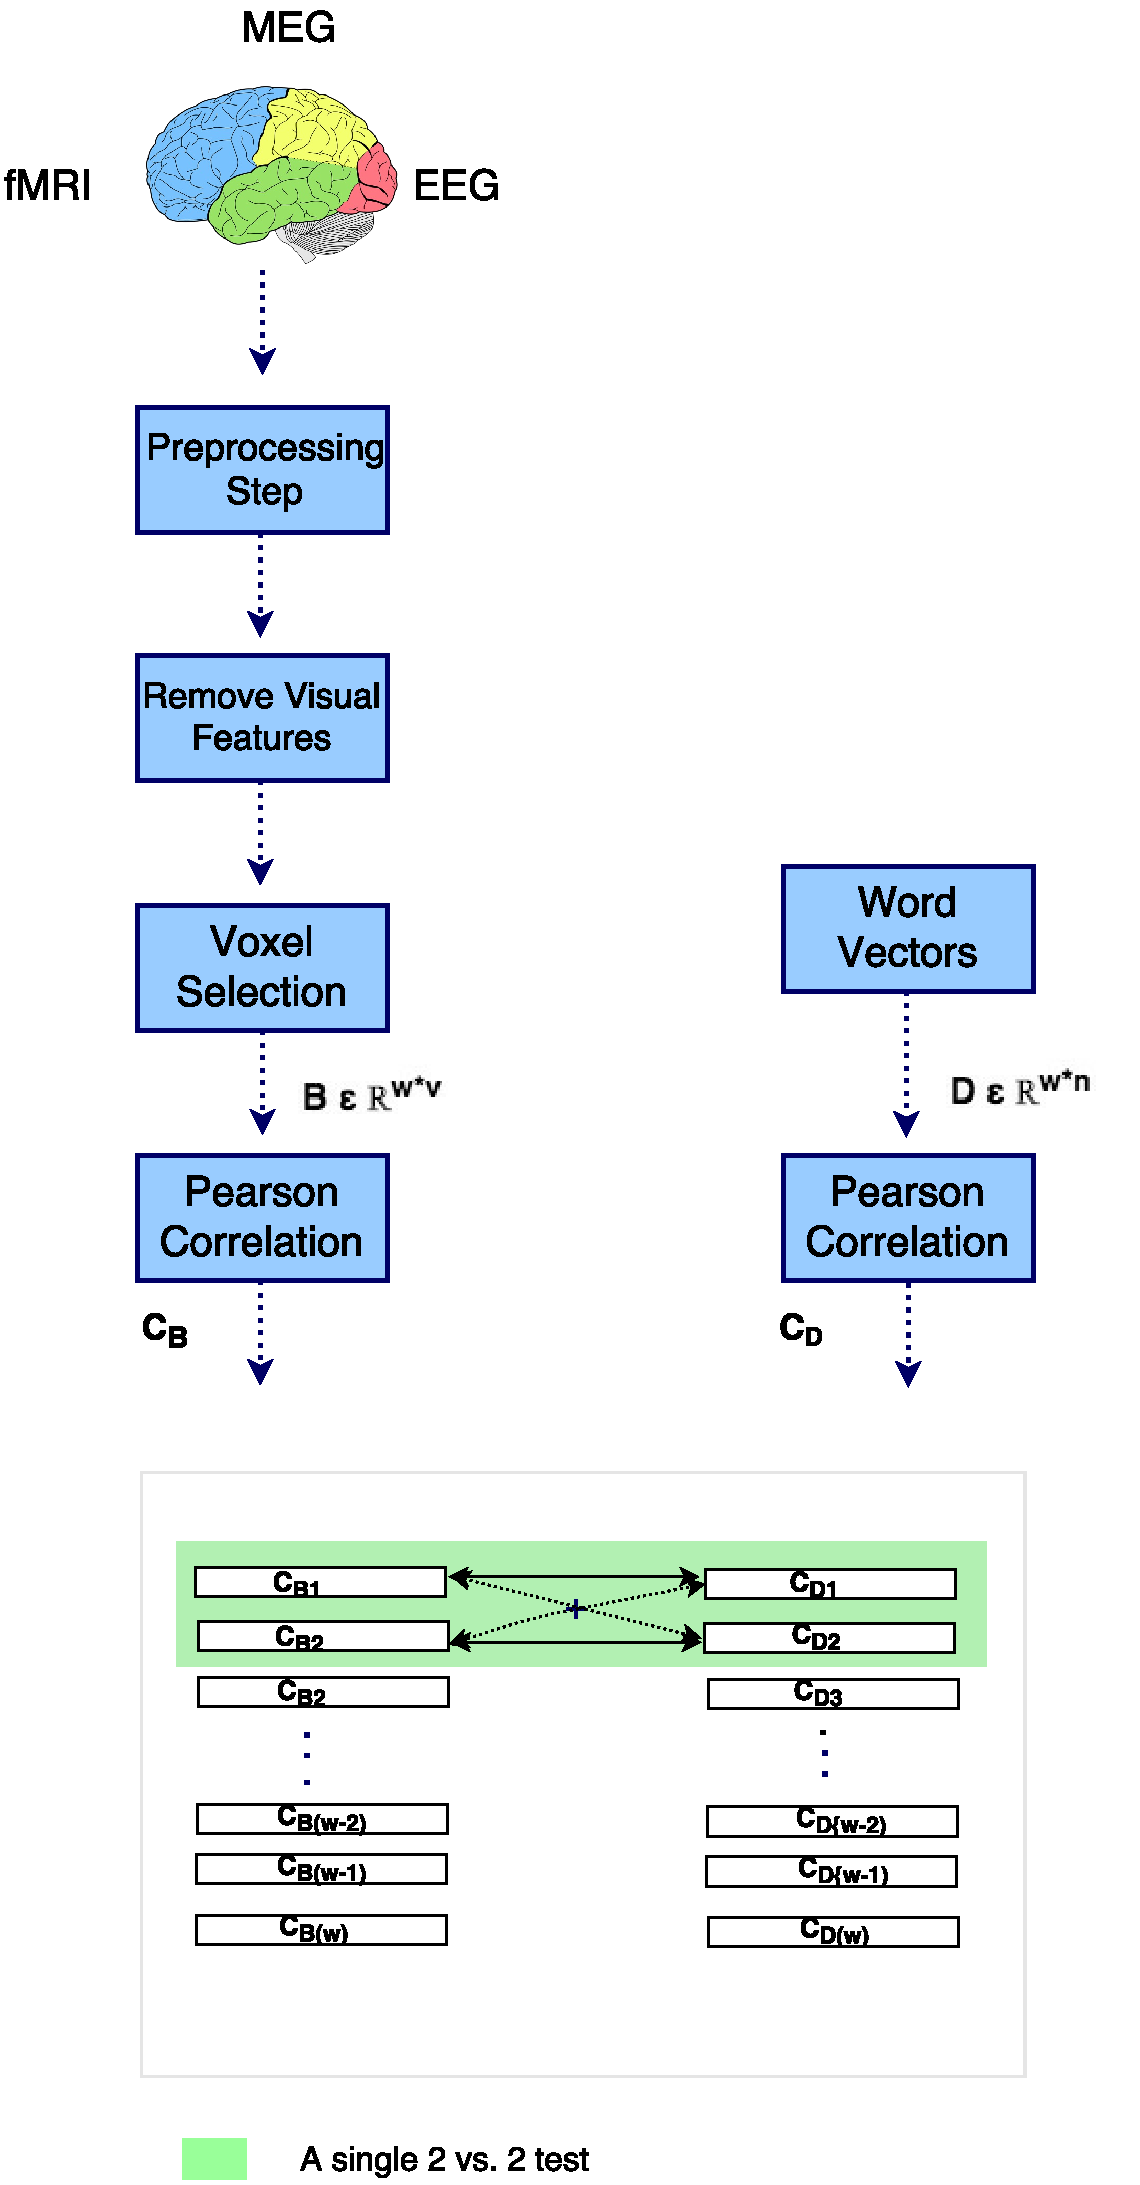
\includegraphics[width=10cm, height=20cm]{Figures/BrainBenchDiagram1}
\caption{A flow diagram showing the methodology followed in adding a Brain dataset to the test suite.}
\label{BrainBenchMethod}
\end{figure}


The visual features are removed by training a Linear Regression model which predicts a value per voxel corresponding to the visual features in the brain signal. These learned visual features are subtracted from the original brain signal. A linear regression model tries to fit a straight line for a set of data points in such a way that the sum of squared errors is minimal [Figure:~\ref{LinearRegression}].  We learn the weight matrix ($\mathbf w$) which parameterizes the best fit line for every data point $(\mathbf x_i, y_i)$. Let us defines the error $e_i$ as the distance between the true and predicted values such that $e_i = y_i - \mathbf w^T \mathbf x_i$. The objective function of the linear regression model is to minimize the the sum of squared errors such that $\sum e_i^2 =  \| X \mathbf w - \mathbf y \|^2$, where ($\mathbf X$)  in our context are the visual features for each trial in our experiment and $\mathbf y$ is the brain signal. 



\begin{figure}[h]
\centering
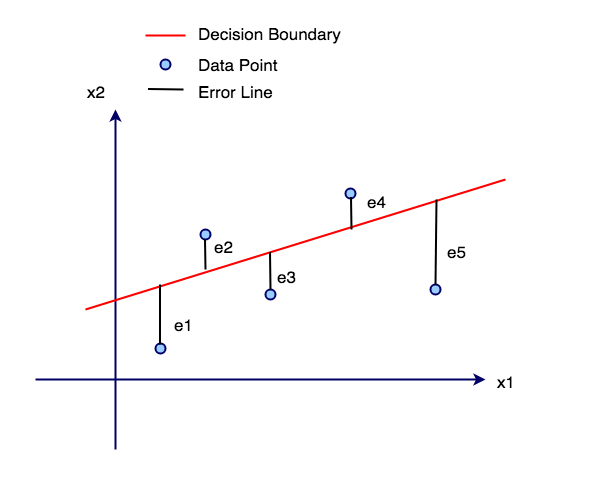
\includegraphics[width=10cm, height=8cm]{Figures/LinearRegression}
\caption{ A Linear Regression model tries to fit a straight line for a set of data points in such a way that the sum of squared errors is minimal.}
\label{LinearRegression}
\end{figure}

Sometimes the visual features might be correlated with one another resulting in a lot of variance across the data. An example could be the length of words could be correlated with the number of black pixels on the screens used to represent the word. This can result in the weight matrix ($\mathbf w$) being poorly  determined and could result in over-fitting. This collinearity between features could cause the $\mathbf w$ to have very large updates for a particular training sample and therefore may not generalize across all other samples in the data. Therefore, we introduce weight decay to restrict the updates to the weight matrix ($\mathbf w$) in the presence of very large coefficients in the feature matrix ($\mathbf X$). This is also known regularization. The objective function of a linear regression model with regularization is given as %
\[\min\limits_{\mathbf w} \| X \mathbf w - y \|^2 + \lambda \, \| \mathbf w \|^2\]

where $\lambda$ is the regularization parameter which is a hyper-parameter and is learned by the model for each dataset separately. The regularization followed here is also knows as L2 normalization. The $\lambda$ is directly multiplied with the square of the weight matrix ($\mathbf w$). Squaring a number punishes large values more than it punishes small values. This implies that large updates to the weights are more penalized than the small updates. The learned weight matrix ($\mathbf w$) represents the signal corresponding to the visual features in the brain data. This weight matrix ($\mathbf w$) is then subtracted from brain signal ($\mathbf y$) to remove the visual features. This method is also termed as ”partialling out” an effect.

The brain data after the removal of visual features is still correlated with noise. We followed the same methodology used by Michell et al. \cite{Mitchell1191} to select the most stable voxels. In this process, we select only those voxels which show strong self correlation across various trails of the same word. The voxels which have such strong self correlations would have a high stability score. Here, we assume that any voxel with a low stability score could be correlated with noise and are not considered for our experiments. Roughly, around 10\% of voxels from each dataset were selected and used in our study.

The brain data corresponding to repetitions of the same word are then averaged for each participant resulting in a matrix $\ B\in \mathbb{R} ^{w*v}$,where $w$ is the number of words and $v$ is the number of voxels selected. We then calculate the Pearson correlation of every word in brain data with every other word resulting in the brain correlation matrix ($C_B$) where $\ C_B\in \mathbb{R} ^{w*w}$. Every row $C_{B_i}$ of the matrix $C_B$ represents the correlation of the word $i$ with every other word from $1$ to $w$ in the brain dataset. 

The same approach is followed for the DS models. From each DS model we extract the words that are present in the model and the brain datasets resulting in the matrix $\ D\in \mathbb{R} ^{w*n}$, where $w$ is the number of words and n is the number of dimension of the word vector. We then compute the Pearson correlation of every word in word vector matrix $D$ with every other word in the matrix resulting in the correlation matrix $C_D$ where $\ C_D\in \mathbb{R} ^{w*w}$ .

Now we have created two correlation matrices $C_B$ and  $C_D$ representing similarity of words in different vector spaces. We could use the Representational Similarity Analysis (RSA) method to compute the correlation between matrices $C_B$ and  $C_D$ \cite{RSA}. RSA is a simple method adopted from the field of neuroscience to study the relationship between two vector spaces. However, the RSA has a disadvantage that it produces one aggregate score for the relationship between two matrices. Sometimes it becomes important to study and understand the parts of the correlation matrix which may result in a high or low score. 

Instead of measuring the correlation between the matrices $C_B$ and  $C_D$ using RSA, we perform the 2 vs. 2 test derived from the early works of Michell et al. searching for word embeddings in the brain \cite{Mitchell1191}. This methodology introduced by  Anderson et al. \cite{Andrew2vs2} and Xu et al. \cite{BrainBench2016} could be considered as a extension of RSA with the 2 vs. 2 test. In 2 vs. 2, we select the columns corresponding to two concepts ($c_1$ and $c_2$) from our correlation matrices $C_B$ and  $C_D$. We then omit the rows corresponding to two concepts resulting in a reduced vector with $w-2$ rows from both the matrices where $w$ is the total number of concepts. These vectors represent the similarity of the two concepts with every other concept except for their self correlation \{corr($c_1$~,$c_1$) and~corr($c_2$~,$c_2$)\} and their correlation with one another \{corr($c_1$~,$c_2$) and~corr($c_2$~,$c_1$)\}. Lets call the reduced vectors as
$C_{B_1}$, $C_{B_2}$ from correlation matrix $C_B$ and $C_{D_1}$, $C_{D_2}$ from correlation matrix $C_D$. The correlation of the concepts $c_1$ and $c_2$ from $C_B$ and  $C_D$  are then computed to check if the correlation of the correctly matched pairs:

\[corr(C_{B_1},C_{D_1}) + corr(C_{B_2},C_{D_2})  \]

\noindent is greater than the correlation of the mismatched pairs:

\[corr(C_{B_1},C_{D_2}) + corr(C_{B_2},C_{D_1})  \]

A 2 vs. 2 test is considered to be passed if the correlation of the matched pairs is greater than correlation of the mismatched pairs. The test is repeated for all possible pairs of concepts in our dataset. This results in $^wC_2$ tests for a dataset with $w$ concepts. The 2 vs. 2 accuracy is defined as the percentage of 2 vs. 2 passed. The change accuracy is 50\%. To compute the significance of our results, we conduct 1000 permutation tests by randomly shuffling the rows and columns of the correlation matrix $C_D$ and re-running the 2 vs. 2 tests for each permutation.

The methodology described in this section varies from the method described by Xu et al. in the first paper \cite{BrainBench2016}. In the methodology described here, we remove visual features before voxel selection as compared to the previous work where voxel selection was performed before removing visual features from the brain signal. Voxel selection selects the most stable voxels and helps to remove noise from the signal. However, if voxel selection is performed without removing visual features from the signal, the most stable voxels selected could the ones which are correlated with visual features rather than semantics. Therefore, we recommend removing visual features from the signal prior to voxel selection. There is a significance improvement seen in the BrainBench test results due to this small change in process. These results are highlighted under the section \textit{Results and Discussions} of this chapter.

\begin{figure}[h]
\centering
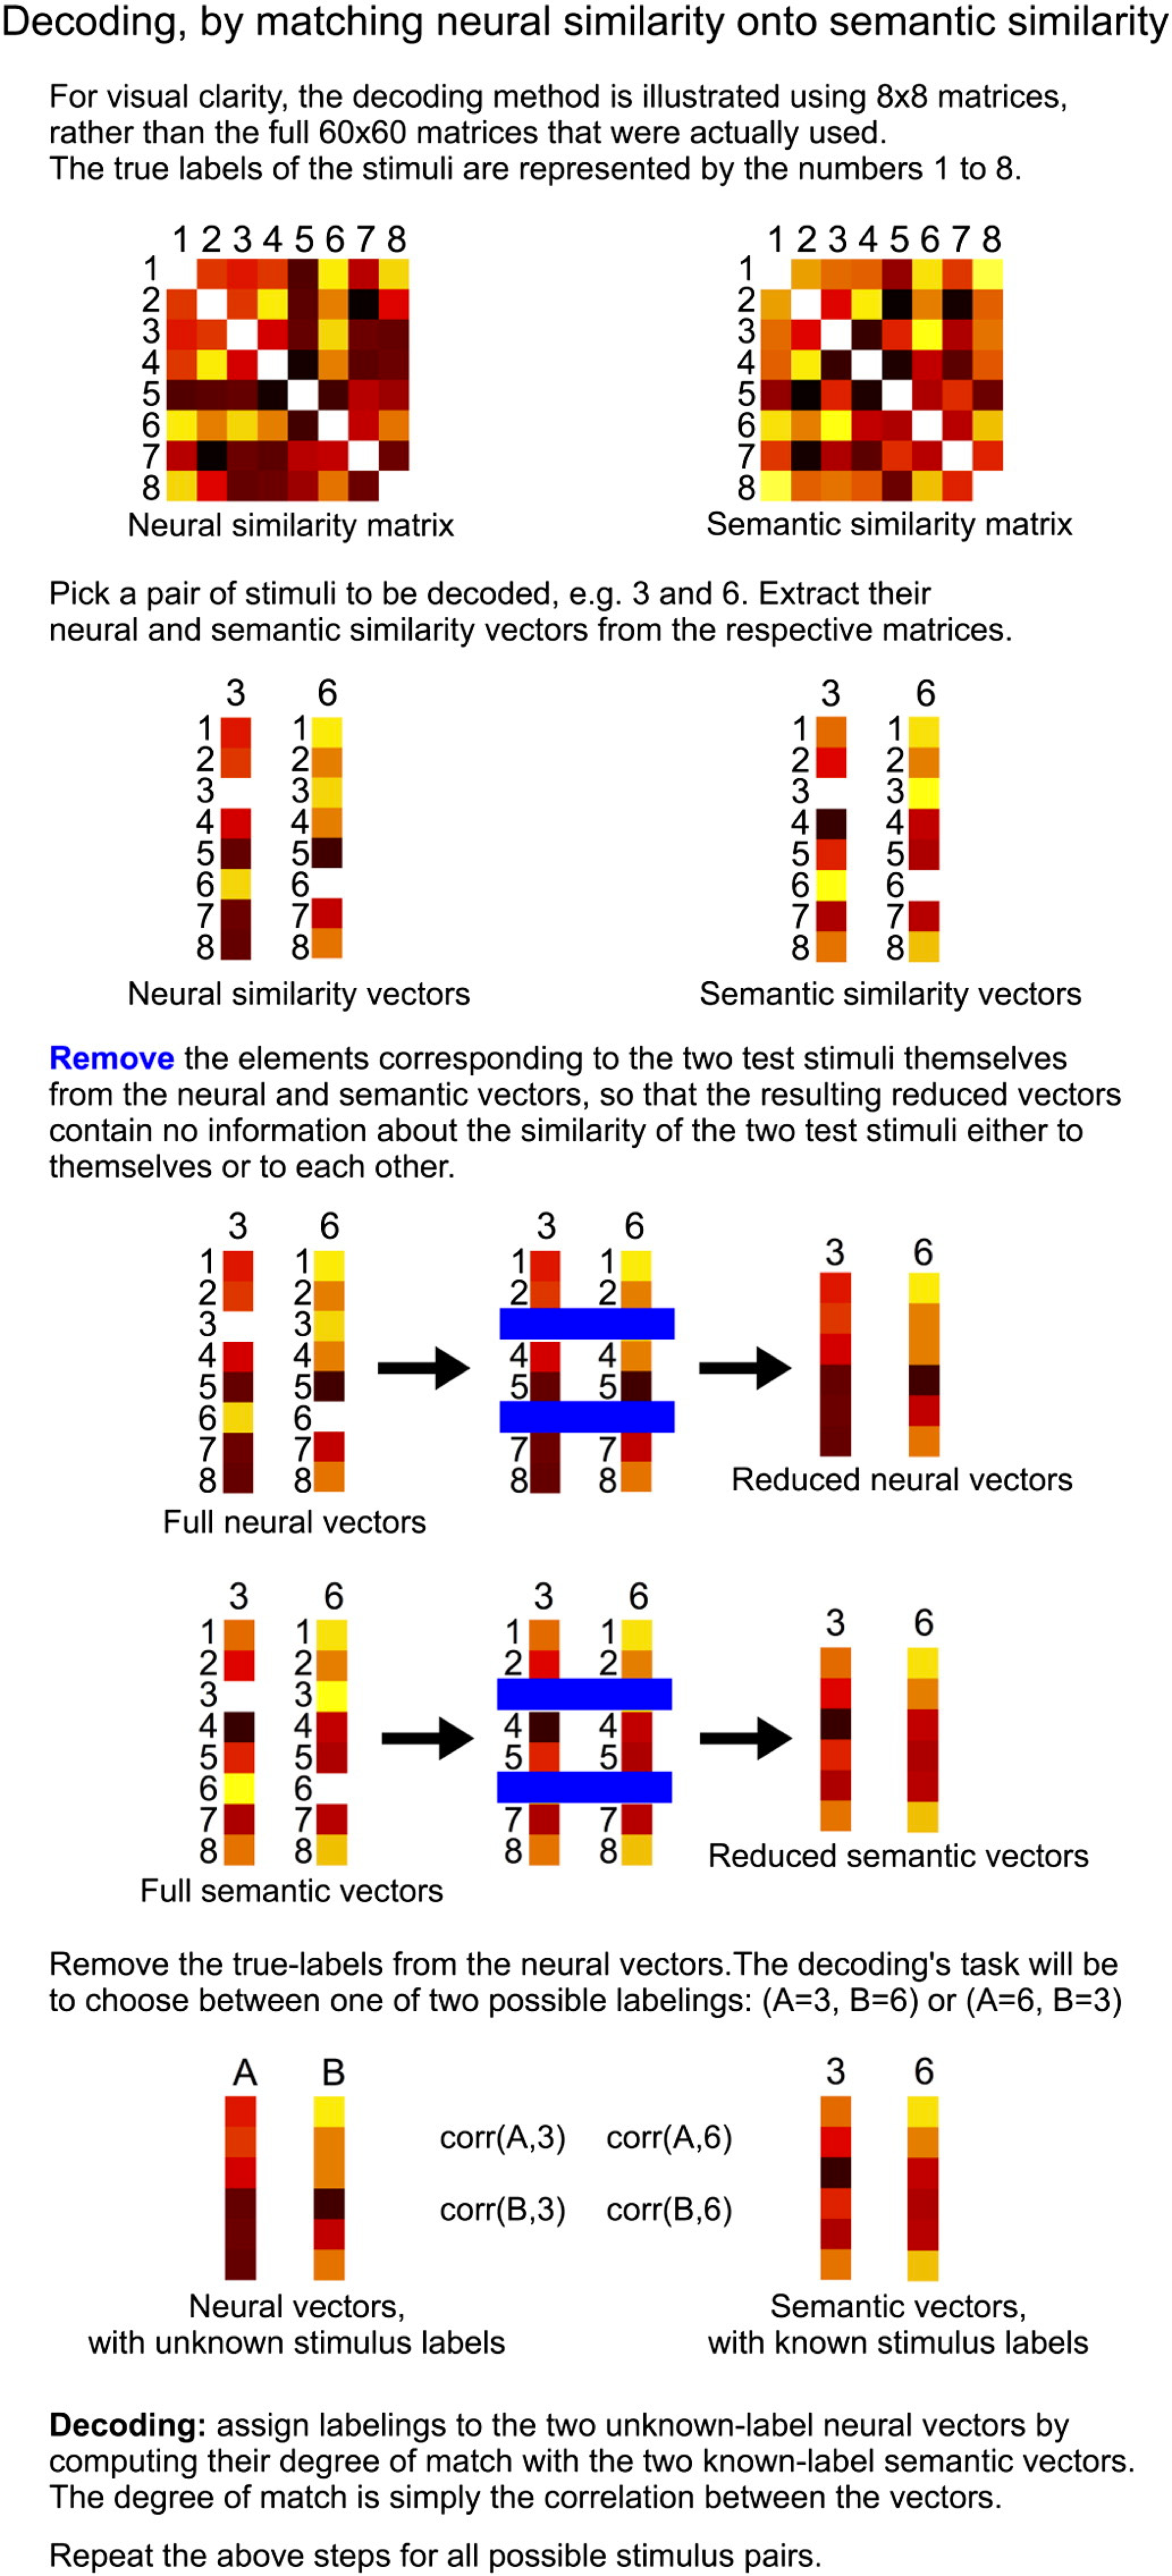
\includegraphics[width=10cm, height=20cm]{Figures/2vs2_anderson}
\caption{ This figure depicts an example of the 2 vs 2 test for 8 words \cite{Anderson2015}.}
\label{2 vs 2}
\end{figure}



\subsection{Concrete Vs Abstract Nouns}

\subsection{Evaluation of Italian word vector}

\subsection{Evaluation against anatomical brain regions}

\section{Results and Discussions}

\section{Summary}


